% !TEX root = rapport_root.tex
\section{Initial Exploration of the Embedding Space}

\subsection{Methods for Visualization: Dimensionality Reduction}

To visualize and interpret the high-dimensional embedding space, we use
\emph{dimensionality reduction} techniques. These methods project the data into
lower dimensional spaces (e.g. 2-dim), aiming to preserve the data's most
essential structural features. We employed three common techniques.

\textbf{Principal Component Analysis (PCA)} is a linear technique meant to
preserve as much global variance as possible. It creates a reduced dataset with
new, fewer variables (principal components). When used for 2D visualization, the
two principal components that capture the most variance are used as the axes
\autocite{IBMndPrincipal}.

\textbf{T-distributed Stochastic Neighbour Embedding (t-SNE)} is a non-linear
approach that excels at preserving the local structure of the data. It focuses
on keeping neighboring data points close to each other in the lower-dimensional
projection, making it highly suitable for identifying clusters
\autocite{Mazraeh2025Comprehensive}.

\textbf{Uniform Manifold Approximation and Projection (UMAP)} is another
non-linear approach that balances the preservation of both local and global
structure. It is often faster than t-SNE and can be more effective at
representing the overarching shape of the data alongside local clusters
\autocite{CoenennpUnderstanding}.

\subsection{Methods for Discovery: Clustering}

To programmatically identify groups in our unlabeled data, we use
\emph{clustering} algorithms. This unsupervised learning technique groups
similar vectors based on their position in the embedding space.

\textbf{K-Means} partitions the data into a pre-defined number of clusters
($k$), assigning each data point to the cluster with the nearest mean or
'centroid'.

\textbf{HDBSCAN} (Hierarchical Density-Based Spatial Clustering of Applications
with Noise) creates clusters based on data density. It identifies regions where
points are tightly packed, making it particularly effective for oddly shaped
clusters and for identifying noise points that don't belong to any cluster
\autocite{Stewart2022Implementation}.

\subsection{Initial Findings from Data Exploration}

To get a general impression of the embedding space, we performed some initial
clustering and dimensionality reduction. Our primary focus was to see if
sections could be distinguished by their function (e.g., ``Methods'',
``Theory''), which would inform our subsequent classification task.

First, we explored how section embeddings relate to the overall theme of their
parent article, using the thematic categories from Lane's analysis. In
Figure~\ref{fig:pca_umap_sections}, we use PCA and UMAP to visualize the
sections, coloring them by theme. As is evident from the distinct groupings, a
section’s location is \emph{heavily dominated by its article's overarching
theme}. This confirms that a section-level approach is needed to analyze
intra-article structure.

\begin{figure}
    \centering
    \begin{subfigure}[b]{0.49\textwidth}
        \centering
        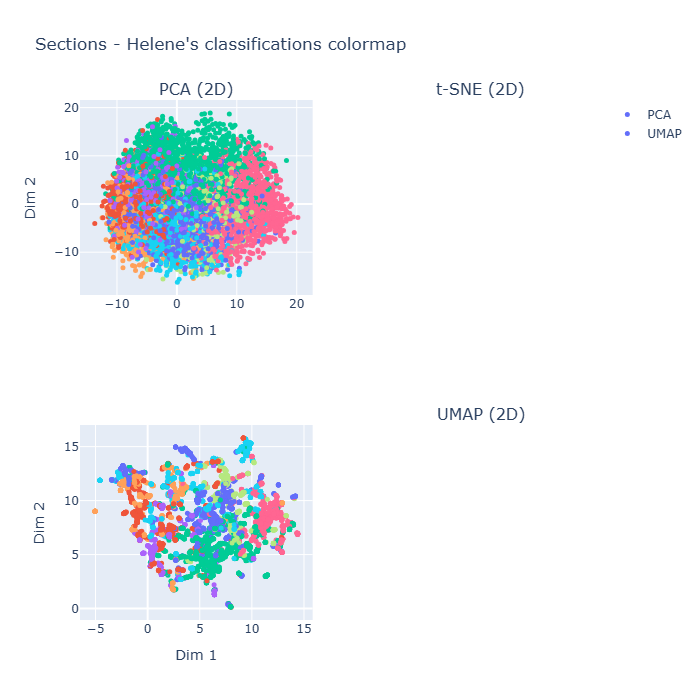
\includegraphics[width=\textwidth]{media/helene_themes.png}
        \caption{Sections colored by article theme (from Lane's analysis).}
        \label{fig:helene_themes}
    \end{subfigure}
    \hfill
    \begin{subfigure}[b]{0.49\textwidth}
        \centering
        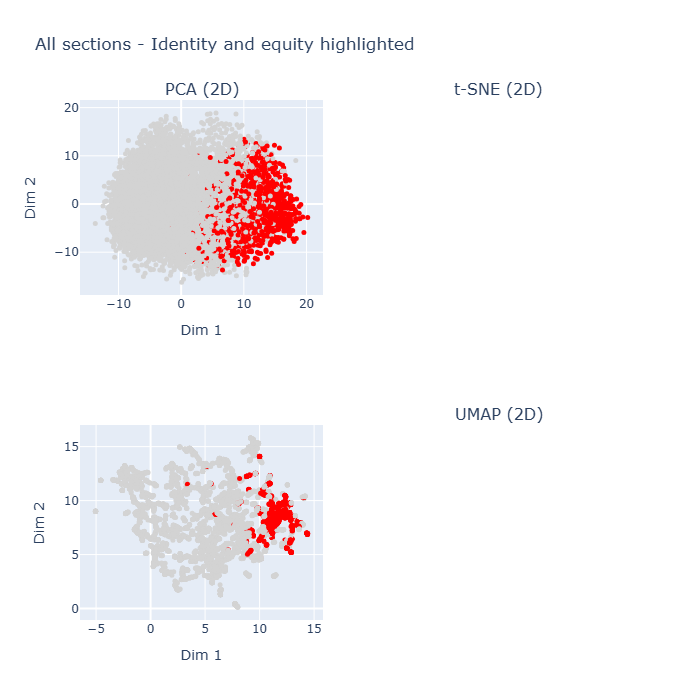
\includegraphics[width=\textwidth]{media/helene_identity_equity.png}
        \caption{Sections from "identity and equity" articles highlighted.}
        \label{fig:identity_highlight}
    \end{subfigure}
    \caption{PCA and UMAP plots of embedded sections, showing strong clustering by article theme.}
    \label{fig:pca_umap_sections}
\end{figure}

Next, we investigated the internal structure within articles.
Figure~\ref{fig:sampled_articles} shows a PCA plot of all sections, with
sections from 9 randomly sampled articles highlighted. While sections from the
same article cluster together, there is meaningful variation between them. This
\emph{intra-article spread} gives us hope that we can exploit this structure for
classification.

\begin{figure}
    \centering
    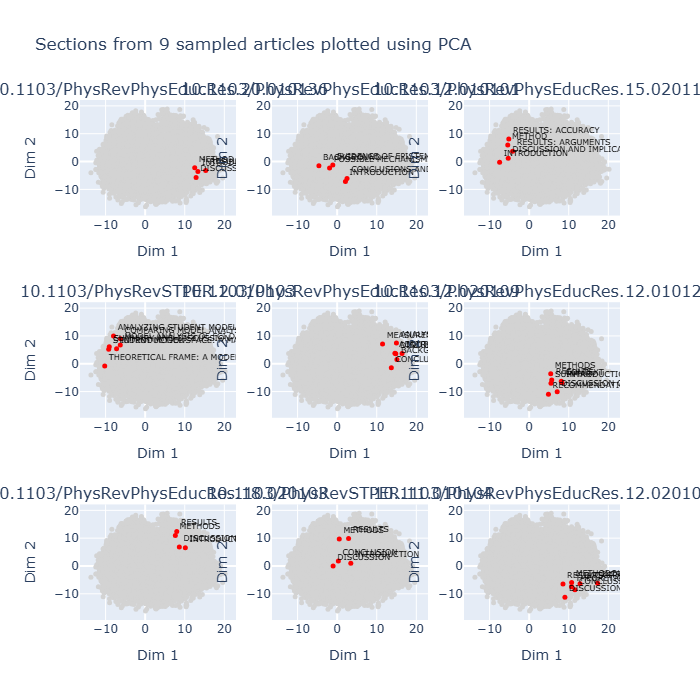
\includegraphics[width=0.7\textwidth]{media/article_sections_structure.png}
    \caption{PCA reduction of all sections with 9 randomly sampled articles highlighted.}
    \label{fig:sampled_articles}
\end{figure}

Finally, we attempted to find natural groupings based on section type using
clustering algorithms (K-Means and HDBSCAN), shown in
Figure~\ref{fig:clustering_comparison}. While the algorithms produced clusters,
these groupings did not correspond to discernible section types. This finding
underscores the \emph{need for more sophisticated, supervised classification
methods}, which we explore in the following section.

\begin{figure}
    \centering
    \begin{subfigure}[b]{0.46\textwidth}
        \centering
        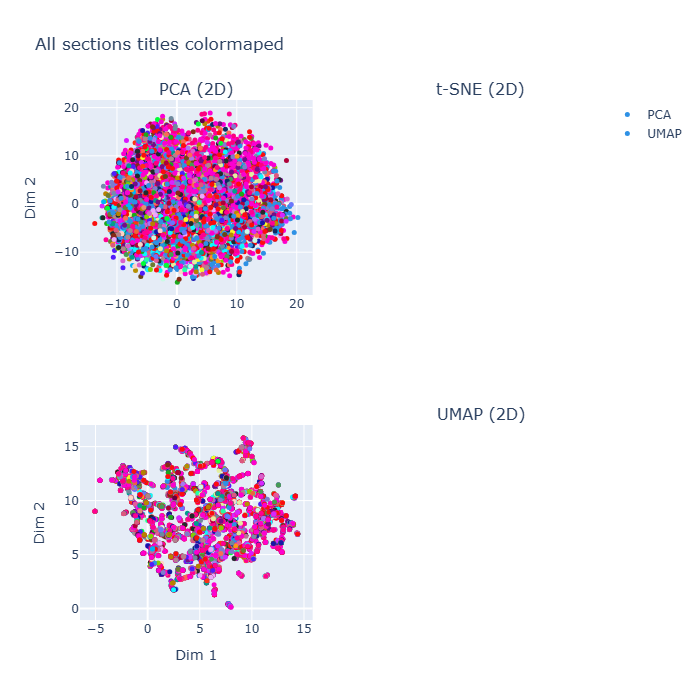
\includegraphics[width=\textwidth]{media/image4.png}
        \caption{K-Means clustering.}
        \label{fig:kmeans_cluster}
    \end{subfigure}
    \hfill
    \begin{subfigure}[b]{0.46\textwidth}
        \centering
        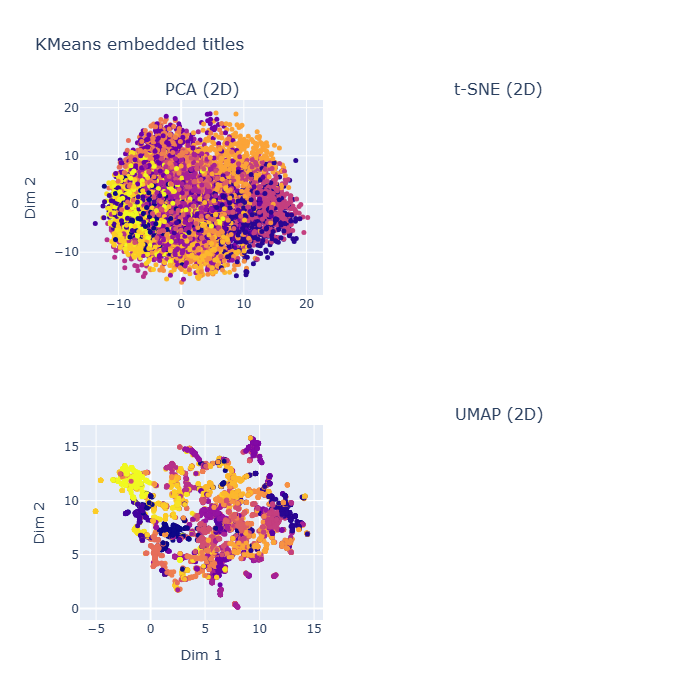
\includegraphics[width=\textwidth]{media/image5.png}
        \caption{HDBSCAN clustering.}
        \label{fig:hdbscan_cluster}
    \end{subfigure}
    \caption{A comparison of clustering algorithms applied to section embeddings. The resulting clusters did not align with section types.}
    \label{fig:clustering_comparison}
\end{figure}

\subsection{Summary of Exploratory Findings}

Our initial exploration of the section embeddings yielded three crucial insights
that shaped the subsequent direction of this project.

First, and most importantly, we found that the \emph{overarching theme of an
article is the dominant factor} determining the location of its sections in the
embedding space. Sections from articles about ``quantum physics'' cluster
together, far from sections from articles about ``identity and equity''. This
presents a significant challenge, as the thematic signal could easily overwhelm
the more subtle signal of a section's function when attempting to classify
section types.

Second, despite this strong thematic clustering, we observed a \emph{meaningful
intra-article structural variance}. Sections within the same article are not
identical points; they occupy a distinct region in the space, which suggests
that their different functions can potentially be distinguished. This finding
provides the basis for our project's feasibility.

Finally, our attempts to use unsupervised clustering algorithms to automatically
group sections by type (e.g., all `Methods` sections) were unsuccessful. This
demonstrates that while structural differences exist, they are not easily
separable.

This conclusion motivates the work of the following chapter, where we develop
and evaluate supervised models specifically designed for this classification
task.